\documentclass{article}
\usepackage{tikz}

\begin{document}

\begin{figure}[h]
    \centering
    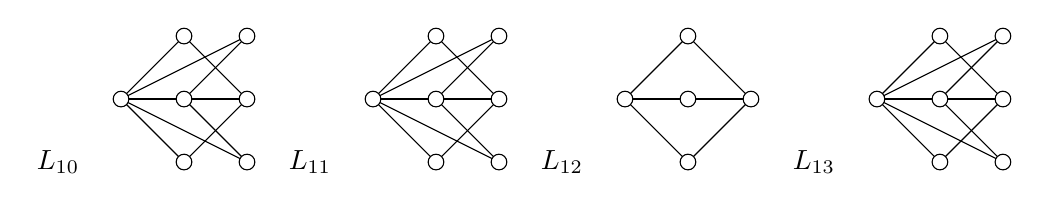
\begin{tikzpicture}[scale=0.8]
        % L_{10}
        \draw (0,0) -- (1,1) -- (2,0) -- cycle;
        \draw (0,0) -- (1,-1) -- (2,0) -- cycle;
        \draw (0,0) -- (1,0) -- (2,0) -- cycle;
        \draw (0,0) -- (1,0) -- (2,1) -- cycle;
        \draw (0,0) -- (1,0) -- (2,-1) -- cycle;
        
        \node at (0,0) [circle, draw, fill=white, inner sep=2pt] {};
        \node at (1,1) [circle, draw, fill=white, inner sep=2pt] {};
        \node at (2,0) [circle, draw, fill=white, inner sep=2pt] {};
        \node at (1,-1) [circle, draw, fill=white, inner sep=2pt] {};
        \node at (1,0) [circle, draw, fill=white, inner sep=2pt] {};
        \node at (2,1) [circle, draw, fill=white, inner sep=2pt] {};
        \node at (2,-1) [circle, draw, fill=white, inner sep=2pt] {};
        
        \node at (-1,-1) {$L_{10}$};
        
        % L_{11}
        \begin{scope}[xshift=4cm]
            \draw (0,0) -- (1,1) -- (2,0) -- cycle;
            \draw (0,0) -- (1,-1) -- (2,0) -- cycle;
            \draw (0,0) -- (1,0) -- (2,0) -- cycle;
            \draw (0,0) -- (1,0) -- (2,1) -- cycle;
            \draw (0,0) -- (1,0) -- (2,-1) -- cycle;
            
            \node at (0,0) [circle, draw, fill=white, inner sep=2pt] {};
            \node at (1,1) [circle, draw, fill=white, inner sep=2pt] {};
            \node at (2,0) [circle, draw, fill=white, inner sep=2pt] {};
            \node at (1,-1) [circle, draw, fill=white, inner sep=2pt] {};
            \node at (1,0) [circle, draw, fill=white, inner sep=2pt] {};
            \node at (2,1) [circle, draw, fill=white, inner sep=2pt] {};
            \node at (2,-1) [circle, draw, fill=white, inner sep=2pt] {};
            
            \node at (-1,-1) {$L_{11}$};
        \end{scope}
        
        % L_{12}
        \begin{scope}[xshift=8cm]
            \draw (0,0) -- (1,1) -- (2,0) -- cycle;
            \draw (0,0) -- (1,0) -- (2,0) -- cycle;
            \draw (0,0) -- (1,-1) -- (2,0) -- cycle;
            
            \node at (0,0) [circle, draw, fill=white, inner sep=2pt] {};
            \node at (1,1) [circle, draw, fill=white, inner sep=2pt] {};
            \node at (2,0) [circle, draw, fill=white, inner sep=2pt] {};
            \node at (1,0) [circle, draw, fill=white, inner sep=2pt] {};
            \node at (1,-1) [circle, draw, fill=white, inner sep=2pt] {};
            
            \node at (-1,-1) {$L_{12}$};
        \end{scope}
        
        % L_{13}
        \begin{scope}[xshift=12cm]
            \draw (0,0) -- (1,1) -- (2,0) -- cycle;
            \draw (0,0) -- (1,0) -- (2,0) -- cycle;
            \draw (0,0) -- (1,-1) -- (2,0) -- cycle;
            \draw (0,0) -- (1,0) -- (2,1) -- cycle;
            \draw (0,0) -- (1,0) -- (2,-1) -- cycle;
            
            \node at (0,0) [circle, draw, fill=white, inner sep=2pt] {};
            \node at (1,1) [circle, draw, fill=white, inner sep=2pt] {};
            \node at (2,0) [circle, draw, fill=white, inner sep=2pt] {};
            \node at (1,0) [circle, draw, fill=white, inner sep=2pt] {};
            \node at (1,-1) [circle, draw, fill=white, inner sep=2pt] {};
            \node at (2,1) [circle, draw, fill=white, inner sep=2pt] {};
            \node at (2,-1) [circle, draw, fill=white, inner sep=2pt] {};
            
            \node at (-1,-1) {$L_{13}$};
        \end{scope}
    \end{tikzpicture}
\end{figure}

\end{document}